\documentclass[
  digital, %% The `digital` option enables the default options for the
           %% digital version of a document. Replace with `printed`
           %% to enable the default options for the printed version
           %% of a document.
  color,   %% Uncomment these lines (by removing the %% at the
           %% beginning) to use color in the digital version of your
           %% document
  table,   %% The `table` option causes the coloring of tables.
           %% Replace with `notable` to restore plain LaTeX tables.
  %twoside, %% The `twoside` option enables double-sided typesetting.
           %% Use at least 120 g/m² paper to prevent show-through.
           %% Replace with `oneside` to use one-sided typesetting;
           %% use only if you don’t have access to a double-sided
           %% printer, or if one-sided typesetting is a formal
           %% requirement at your faculty.
  oneside, % temp for digital version
  lof,     %% The `lof` option prints the List of Figures. Replace
           %% with `nolof` to hide the List of Figures.
  lot,     %% The `lot` option prints the List of Tables. Replace
           %% with `nolot` to hide the List of Tables.
  %% More options are listed in the user guide at
  %% <http://mirrors.ctan.org/macros/latex/contrib/fithesis/guide/mu/fi.pdf>.
]{fithesis3}
%% The following section sets up the locales used in the thesis.
\usepackage[resetfonts]{cmap} %% We need to load the T2A font encoding
\usepackage[T1,T2A]{fontenc}  %% to use the Cyrillic fonts with Russian texts.
\usepackage[
  main=english, %% By using `czech` or `slovak` as the main locale
                %% instead of `english`, you can typeset the thesis
                %% in either Czech or Slovak, respectively.
  czech         %% The additional keys allow
]{babel}        %% foreign texts to be typeset as follows:
%%
%%   \begin{otherlanguage}{czech}   ... \end{otherlanguage}
%%
%% The following section sets up the metadata of the thesis.
\thesissetup{
    date        = \the\year/\the\month/\the\day,
    university  = mu,
    faculty     = fi,
    type        = bc,
    author      = Jan Rychlý,
    gender      = m,
    advisor     = {doc. Mgr. Jan Obdržálek, PhD.},
    title       = {Game development in Haskell},
    % TeXtitle    = {Game development in Haskell},
    keywords    = {Haskell, functional paradigm, game development, Apecs},
    % TeXkeywords = {keyword1, keyword2, \ldots},
    abstract    = {%
      This is the abstract of my thesis, which can

      span multiple paragraphs.
    },
    thanks      = {%
      These are the acknowledgements for my thesis, which can

      span multiple paragraphs.
    },
    bib         = bibliography.bib,
    %% Uncomment the following line (by removing the %% at the
    %% beginning) and replace `assignment.pdf` with the filename
    %% of your scanned thesis assignment.
%%    assignment         = assignment.pdf,
}
\usepackage{makeidx}      %% The `makeidx` package contains
\makeindex                %% helper commands for index typesetting.
%% These additional packages are used within the document:
\usepackage{paralist} %% Compact list environments
\usepackage{amsmath}  %% Mathematics
\usepackage{amsthm}
\usepackage{amsfonts}
\usepackage{url}      %% Hyperlinks
\usepackage{markdown} %% Lightweight markup
\usepackage{tabularx} %% Tables
\usepackage{tabu}
\usepackage{booktabs}

\usepackage[newfloat, chapter]{minted} %% source code highlighting
\usemintedstyle{vs}
\usepackage{xcolor}
\usepackage{hyperref}
\usepackage{dirtytalk}

\usepackage{floatrow} %% Putting captions above tables
\floatsetup[table]{capposition=top}



% C++ macros
\newcommand{\cpp}{C\nolinebreak\texttt{+}\nolinebreak\texttt{+}}
\newminted[cppblock]{cpp}{breaklines}
\newmintinline[inlinecpp]{cpp}{breaklines}

% Haskell macros
\definecolor{haskellbg}{rgb}{0.95,0.95,0.96}
\newminted[haskell]{haskell}{
    % frame = leftline,
    % bgcolor = haskellbg,
    breaklines,
    % breakanywhere,
    % escapeinside=//,
}
\newmintinline[inlinehs]{haskell}{breaklines}
\newcommand{\packagename}{\mintinline{Haskell}}

\newminted[term]{console}{breaklines}

\newcommand{\vs}{vs.\ }




\begin{document}


% ====================================
% Introduction
% ====================================
\chapter*{Introduction}
\addcontentsline{toc}{chapter}{Introduction}
\label{chptr:introduction}

% // introduction draft written for the VB000 assignment

Video games are a special kind of application that many consider an art form
and rewarding to develop. However, they generally involve a complex system
with a non-trivial state, a certain amount of pseudo-randomness,
and user/player input handling. This makes for non-deterministic
programs that are usually incredibly difficult to test efficiently.

Conversely, functional programming strives to eliminate
mutable state and make code more deterministic, which allows for
programs to be safer and easier to test.
These and other benefits have naturally led to people
trying out game development in functional languages, but
it remains mostly a matter of passion projects.
That said, even though the vast majority of the video game industry
still uses imperative languages like \cpp{}, the communities
\emph{are} very active, and there are hundreds of games,
blog posts, and libraries that help with
game programming in functional languages.

The focus of this thesis narrows down to exploring game development
in Haskell in the context of small-scale 2D games. The goal is
to give an overview of the process, then compare this approach
to a more conventional and imperative one
and ultimately highlight the features of Haskell that are beneficial
and those that become hurdles in the context of programming a video game.

This is done through reimplementing a single game with an already existing
imperative implementation in Haskell,
first using the Apecs\footfullcite{apecsrepo} library
and for a second time without it. After a further discussion
about chosen technologies in the following chapter,
said three implementations are described and analyzed
in chapters 2, 3, and 4. Then they are more closely compared
and the pros and cons of Haskell in game development are
evaluated and demonstrated in chapter 5.

We find that the Apecs library makes developing games
in Haskell much more approachable. On the other hand
it goes against the functional philosophy, and using it
will generally result in very imperative code wrapped in monads
that lacks the expressiveness and apparent safeness of regular Haskell.
Yet, from the second reimplementation, we learn that
some use of monads is beneficial, and it makes the code cleaner
and more elegant. In both cases, the development was
mostly a smooth experience without a single major hiccup,
unlike what often happens when dealing with a \cpp{} compiler.
% Furthermore, from our
% small scale example, it appears that a more \say{pure} architecture allows
% for parallel computation resulting in better performance than an Entity
% Component System like Apecs or the one inside of Unity.\footnote{
% Disclaimer: this is only my incomplete guess of the results,
% the thesis is not yet finished.
% }


% ! be more brief !

% ====================================
% CHAPTER 1 - Deeper introduction
% ====================================
\chapter{Motivation and used methods}
\label{chap:motivationandmethods}


\section{Why functional programming matters}
\label{sect:whyfpmatters}

Functional languages are a subset of declarative languages, where the
programmer states \say{what} instead of \say{how}. Unlike in imperative languages,
we \emph{declare} what we want a program to return by combining functions (other declarations)
instead of giving the computer serialized instructions (\emph{imperatives}).
That is manifested in the lack of assignment statements and lesser control structures.
Once variables are assigned their value, it can't be changed,
and the \say{burden} of prescribing the flow of control
is removed.\cite{whyfpmatters} Moreover, a pure function has no side effects
and its return value depends solely on its arguments. This makes for deterministic
programs that are easier to test, debug and argue about their correctness.

John Hughes describes the key benefits of functional paradigm in his paper
\textit{Why Functional Programming Matters}.\cite{whyfpmatters} He first
explains how modularity of code is clearly very important, since
separate modules are easier to write and test and then proceeds
to show how functional programming increases modularity
through higher-order functions and lazy evaluation, demonstrating
their importance on several examples.

Additionally, Haskell is a purely functional programming language that
is also \emph{strongly typed}. This means that one
doesn't need to worry about memory errors causing crashes because
everything is caught by the type-checker during compilation.
The types also serve as documentation and can help greatly
with writing and understanding code. At the same time,
types can also be inferred by the compiler so it
is not necessary to explicitly declare the type of everything.
Furthermore the type system allows extensive user-defined data types,
which makes the code even more expressive.
All of this potentially increases productivity of a functional programmer even further.


\subsection{Game development specifics}
Functional languages are great tools but we know that not every tool is
fit for every task. One of the consequences of the functional purity is
that the state of the program has to be modeled explicitly as an argument
and is therefore immutable. There are monads that help us abstract
from this but the monads themselves are in a way still an explicit workaround.

Conversely, games are real-time, interactive applications simulating
often very complex systems and hold a non-trivial state that is
updated many times a second. Such state generally involves a representation
of the game world with all the objects existing in it, their properties and flags,
the current state of the input devices and many other variables. Since its beginning,
the video game industry has been dominated by imperative languages,
that make it easy to model a game world and alter it globally through
references and side effects inside of decomposed functions. And because
of their established position, there is a plethora of libraries and game engines
with supporting documentation and tutorials. Besides, a company will most likely
have no problem finding skilled \cpp{} programmers with interest
in the game industry, whereas finding their functional counterparts
might be much harder. Additionally, in the case of \cpp{} the performance
also fits the requirements of large games.

However, it does come with a price --- modules of such programs may be
more dependent and entangled, which makes the whole less flexible and with
implicit state more prone to bugs and harder to test and debug.
That is, while testing is already a large issue due to the nature of video games.
Automated testing is not sufficient and companies have to hire teams
of game testers to test games manually. And in terms of high performance,
which is generally connected to lower-level languages, developers must
wrestle with the lower-level nature, producing problems as well.
Haskell also has the edge in the area of parallelism and concurrency,
which is becoming more relevant as new hardware keeps increasing in core counts,
and complex, intertwined, imperative systems are difficult to run in parallel.

We can see that video games, like any other software, could benefit from
purely functional design, provided that we are able to model the
game state efficiently enough. Another consideration in the real world
are the available frameworks and whether the cost of potential
pioneering is worth to us.


\subsection{Existing work}
Indeed, people have tried developing games in Haskell and a decent
progress has been made over the years. There are libraries/engines like Yampa\cite{yamparepo}
and Helm\cite{helmrepo} for functionally reactive programming (FRP) of video games and
other general FRP libraries that have been used to make games like Elerea\cite{elerearepo}
or Netwire\cite{netwirerepo}. From non-FRP libraries there is
FunGEn\cite{fungenrepo}, the self-proclaimed oldest Haskell game engine,
Apecs\cite{apecsrepo}, which we use to program a game and describe the process
in chapter~\ref{chptr:hasteroids}, and many others. It is important to note that
most of these libraries or engines provide only limited capabilities
compared to \say{real} industry engines like Unity or Unreal Engine
and depending on the type and scale of the game, there is still a lot
of work left for the developer.

Regarding existing games themselves, there are two --- Magic Cookies and
Enpuzzled --- that have been commercially pulished by Keera Studios,
who also stand behind the Yampa game engine\cite{keerastudios}.
Then there is Chucklefish, indie game developer studio, publisher and
creator of popular Starbound, which announced to be working on their next
game Wayward Tide in Haskell back in 2014\cite{waywardtide}. However, there
has not been an announcement of the release date as of 2021 and the studio is
focusing on other projects at the moment.

So it remains to be a pioneering process and the games made are nowhere close
to the rest of the industry but there \emph{is} more games than just the stated few.
They are created by passionate individuals and shared with the community. Dozens of them can be found
on the Haskell game development Reddit page\footnote{
Subreddit about game development in Haskell: \url{http://www.reddit.com/r/haskellgamedev/}
}
for instance. Many have also written blog posts or tutorials alongside with
their games like Joe Vargas and his \textit{A Game in Haskell - Dino Rush}\cite{dinorush},
which goes in-depth and explains his well though out architecture,
or Ashley Smith and her \textit{Of Boxes and Threads: Games development in Haskell}\cite{aashaskell}
and \textit{An Introduction to Developing games in Haskell with Apecs}\cite{aasapecs},
that provide great overview and inspiration.


\section{Rendering and interfacing with the OS}
\label{sect:aboutsdl}
Essential part of a game engine is communicating with the operating system
and rendering of models or textures. To do this we can
either use a complete engine like the before mentioned Helm or
a library built for this purpose like Gloss\cite{?}, which aims to provide an easy to use
interface for managing input and rendering. Other libraries
provide only Haskell bindings to existing media frameworks like GLUT, GLFW and SDL
(Gloss actually uses GLUT or GLFW for its backend). The main goal of these libraries is
to abstract from a specific window system and graphics hardware, providing
cross-platform APIs for rendering, managing windows and receiving input and events.

In both experiments described in this thesis we use the SDL bindings
to load textures and fonts, to poll input events, create windows and render scenes.
Specifically, we use the \packagename{sdl2}, \packagename{sdl2-image}
and \packagename{sdl2-ttf} packages. We chose SDL because there are already
examples of its use in games we can learn from,
the underlying C library works across multiple platforms,
is well documented\footnote{
    The documentation of the C library: \url{https://wiki.libsdl.org/}
} and is widely used. Moreover, the Haskell library
include both high-level and low-level bindings, meaning we can
enjoy a comfortable interface, yet at the same time the
lower-level bindings serve as an example of
the powerful Foregin Function Interface (FFI), which
makes Haskell even more useful in the real world.

Here are the most essential \inlinehs{SDL} functions we use in our two games,
all examples of the high-level bindings:
\begin{itemize}[\textendash]
    \item \inlinehs{SDL.createWindow} used to create a new window,
    \item \inlinehs{SDL.createRenderer} used to create a rendering
    context for a window,
    \item \inlinehs{SDL.Font.load} for loading fonts, 
    \item \inlinehs{SDL.Image.loadTexture} for loading images as textures,
    \item \inlinehs{SDL.clear}, which clears the rendering target/context,
    \item \inlinehs{SDL.copy} and \inlinehs{SDL.copyEx} for copying
    our loaded textures to the rendering target like stamping a picture on a canvas,
    \item \inlinehs{SDL.present}, which displays the current state of the target in the window,
    \item \inlinehs{SDL.pollEvents} called to get input events.
\end{itemize}
In listing \ref{lst:ffi} we can see how FFI is used. It shows \inlinehs{SDL.copy},
which wraps around the low-level binding, abstracting from the pointers,
replacing them with Haskell's \inlinehs{Maybe},
and throwing an error instead of the returning a negative value.

\begin{listing}[H]
\caption{Example of FFI binding.\cite{sdlrepo}}
\label{lst:ffi}
\begin{haskell}
-- the C function (https://wiki.libsdl.org/SDL_RenderCopy):
-- int SDL_RenderCopy(SDL_Renderer * renderer,
--                    SDL_Texture * texture,
--                    const SDL_Rect * srcrect,
--                    const SDL_Rect * dstrect);

-- the binding from SDL.Raw.Video
foreign import ccall "SDL.h SDL_RenderCopy"
    renderCopyFFI :: Renderer
                  -> Texture
                  -> Ptr Rect
                  -> Ptr Rect
                  -> IO CInt

-- the wrapper from SDL.Video.Renderer
copy :: MonadIO m
     => Renderer
     -> Texture
     -> Maybe (Rectangle CInt)
     -> Maybe (Rectangle CInt)
     -> m ()
\end{haskell}
\end{listing}



\section{Asteroids by Atari as an example}
\label{sect:whyasteroids}
Asteroids, is an arcade game created by Atari in 1979.
To evaluate Haskell as a language for game development in general
would be a task far beyond the scope a bachelor's thesis. For that reason
we narrow down our focus to smaller two-dimensional games and at the end
only speculate how our findings may scale to larger games.
We chose Asteroids as an example because its world comprises only of
few object types, yet their relationships make the game quite interesting.
It also does not rely on complex graphics, therefore we can focus
on the code implementing the game rules and behaviors.
\begin{figure}
    \begin{minipage}{0.33\textwidth}
        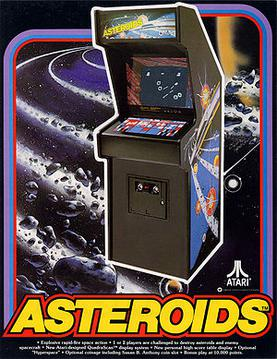
\includegraphics[height=1.3\textwidth]{images/Asteroids-arcadegame.jpg}\hfill
    \end{minipage}
    \hfill
    \begin{minipage}{0.66\textwidth}
        \hfill 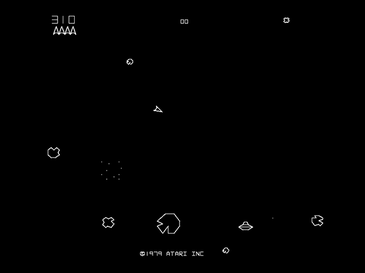
\includegraphics[height=0.65\textwidth]{images/atariasteroids-screenshot.png}
    \end{minipage}
    \caption{Atari Asteroids --- Promotional flyer cover\cite{asteroidsflyer}
    and game-play screenshot.\cite{asteroidsscreenshot}}
    % https://en.wikipedia.org/wiki/File:Asteroids-arcadegame.jpg
    % https://en.wikipedia.org/wiki/File:Asteroi1.png
\end{figure}

The game can be described as followed:
\say{A perfect synergy between simplicity and intense gameplay, the game has players using buttons to thrust a spaceship around an asteroid field. When one rock is shot, it breaks into smaller ones, often flying off in different directions at different speeds\ldots{} Every so often flying saucers enter the screen, intent on the player’s destruction.}\cite{aboutasteroids}
Its world comprises of rocks (asteroids), projectiles,
flying saucers (large or small, trying to shoot the player) and the ship, controlled by the player,
trying to survive and gain score points by shooting down rocks and flying saucers.
There is a few features that we are omitting like sound effects, some animations
and several minor game-play details. But we still need to handle input, simulate simple physics,
detect collisions, spawn entities, keep score, transition between the game
and its menus and then render everything.



% ====================================
% CHAPTER 2 - About Apecs
% ====================================
\chapter{Using the Apecs library --- hAsteroids}
\label{chptr:hasteroids}

\section{About Apecs}
\label{sect:apecs}
\say{Apecs: a fast, type-driven Entity\textendash{}Component\textendash{}System library for game programming,}\cite{apecsrepo}
is one of the more recently released libraries.
Entity\textendash{}Component\textendash{}System (or ECS) is a data-oriented architectural pattern often
used in video game engines to represent the game world state.
In a true ECS, a game object or an \textbf{entity} is only an ID number
and data is attached to it by being stored under that ID. This data is
organized into \textbf{components}, which are then stored in separate
lists with other components of the same type from other entities.\cite{mediumecs} This can
be represented as a table where every column is its own list or array
(see table \ref{tab:ecsexamp}). Then we define game logic as \textbf{systems}
--- set of functions that operate on certain components regardless of the
entity as a whole. A typical example of a system is adding entity's velocity
to its position for every entity that has both of those components.
ECS usually provide better performance than object-oriented designs (OOD)
because of their increased data locality --- a system needs to load into memory
only components that are relevant for it, not the whole \emph{objects}
as it would be with OOD.\cite{apecspaper}
\begin{table}[htp]
  \begin{tabularx}{320pt}{|r|lllX|}
    \toprule
    Entity & Position & Velocity & Type of Unit & Ammunition \\
    \midrule
    0 & $(4,2)$ & $(0,0)$ & Player   & 314\\
    1 & $(5,1)$ & $(1,1)$ & Enemy    & -- \\
    2 & $(2,2)$ & $(1,0)$ & Enemy    & -- \\
    3 & $(2,3)$ & --      & Obstacle & -- \\
    \bottomrule
  \end{tabularx}
  \caption{A simple example of ECS represented by a table.}
  \label{tab:ecsexamp}
\end{table}

And since both Unity and Unreal engine use Entity\textendash{}Component design,
we chose Apecs as the current state-of-the-art Haskell library
for the traction it has received in the community despite
it not being the only ECS library in existence.\footnotemark
\footnotetext{
The making of the Ecstasy library was actually inspired by
author's issues with Apecs as she explains on her blog\cite{whyecstasy}
}

\begin{listing}[H]
\caption{Defining instance of \inlinehs{Component}.}
\begin{haskell}
newtype Position = Position (Double, Double)
instance Component Position where
    type Storage Position = Map Position
\end{haskell}
\label{lst:component}
\end{listing}


To write a game using apecs we must define \textbf{components} and \textbf{systems}.
Systems also take care of creating new \textbf{entities},
as creating them means to store some components under a new ID.

First, defining a \textbf{component} means to define an instance of the class
\inlinehs{Component}, as we see in the listing \ref{lst:component}.
The \inlinehs{Component} class
requires us to state how we want to store the given component
by assigning a type alias to the specific storage type.
We can define our \inlinehs{Stores} or use one of those provided
with the library: \inlinehs{Map}, \inlinehs{Unique}, \inlinehs{Global} (and \inlinehs{Cashe}).
With \inlinehs{Map}, there can be multiple components of that type,
each belonging to a particular entity.
With \inlinehs{Unique}, at most one component may exist
belonging to a particular entity. Furthermore,
with \inlinehs{Global}, at most one component instance can exist,
and it belongs to the special \inlinehs{global} entity together
with every other entity at the same time. Finally, we call \inlinehs{makeWorld},
which uses Template Haskell to generate \inlinehs{World} product type
along with \inlinehs{initWorld} function and instances of the \inlinehs{Has}
class needed for altering contents of \inlinehs{World} through
the other functions in Apecs. The resulting \inlinehs{World}
may look close to something as shown in listing \ref{lst:world}.

\begin{listing}[H]
\caption{Simplified world state type example.}
\begin{haskell}
data World =
    World
    { record1 :: !(Unique Player)
    , record2 :: !(Map Enemy)
    , record3 :: !(Map Bullet)
    , record4 :: !(Map Position)
    , record5 :: !(Global Time)
    }
\end{haskell}
\label{lst:world}
\end{listing}

\textbf{System} in apecs is anything with the \inlinehs{SystemT w m a} return type, which
means that it may alter the world state.
One such \say{micro-system} is the \inlinehs{newEntity} function, which
accepts a tuple of components and adds them into their records under a new ID.
% \begin{haskell}
% newEntity ( Ship $ pi / 2 * 3
%           , Position $ V2 0 0
%           , Velocity $ V2 0 0
%           )
% \end{haskell}
More noteworthy functions to build systems are the component map functions
shown in the listing \ref{lst:cmaps}. They are the means of altering the world state.
\begin{listing}[H]
\caption{Component maps documentation.\cite{apecsdocs}}
\begin{haskell}
-- 'w' is the world type, 'm' is a monad,
-- 'cx','cy' and 'c' are tuples of components

-- | Maps a function over all entities
--   with a cx, and writes their cy.
cmap :: forall w m cx cy.
    (Get w m cx, Members w m cx, Set w m cy) =>
    (cx -> cy) -> SystemT w m ()

-- | Monadically iterates over all entities
--   with a cx, and writes their cy.
cmapM :: forall w m cx cy.
    (Get w m cx, Set w m cy, Members w m cx) =>
    (cx -> SystemT w m cy) -> SystemT w m ()

-- | Monadically iterates over all entities with a cx
cmapM_ :: forall w m c.
    (Get w m c, Members w m c) =>
    (c -> SystemT w m ()) -> SystemT w m ()
\end{haskell}
\label{lst:cmaps}
\end{listing}
\inlinehs{cmap} accepts a function that takes a tuple of components
and returns some other tuple of components. It internally iterates
over entities with at least those components matching the mapped
function's input tuple and writes the output tuple components
to those entities. \inlinehs{cmapM} works similarly
only as its name suggests the mapped function returns the component
tuple wrapped in the system monad, which allows it to execute side effects.
And with \inlinehs{cmaM_} there is no direct writing, only side effects.



\section{Writing of hAsteroids}
\begin{figure}[hbt!]
    \centering
    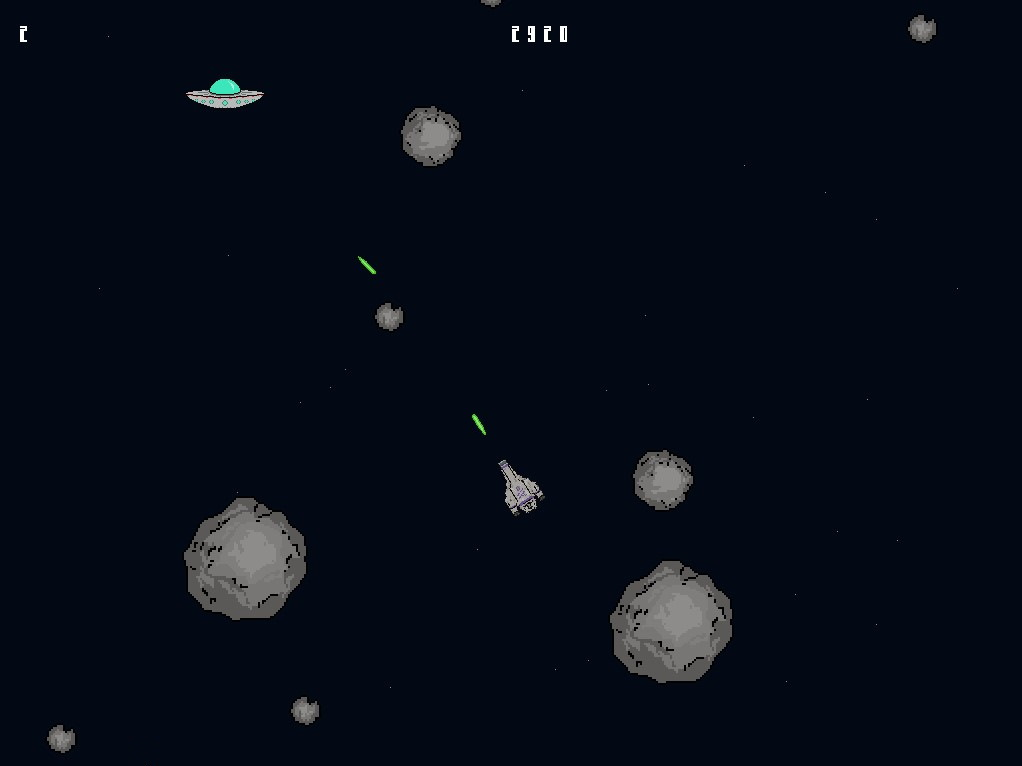
\includegraphics[width=\textwidth]{images/hasteroids-screenshot.jpg}
    \caption{A screenshot of hAsteroids game-play.}
    \label{fig:hasteroidsscreenshot}
\end{figure}

In this section we outline how we used apecs in the hAsteroids game.
For the exact implementation, please refer to the attached source files in the hAsteroids directory.
Figure \ref{fig:hasteroidsmodules} shows project's modules with loosely indicated
dependencies --- upper modules may have direct dependencies on the lower modules,
arrows show most of the important ones. % this miiiighttt be refactored still
\begin{figure}
    \centering
    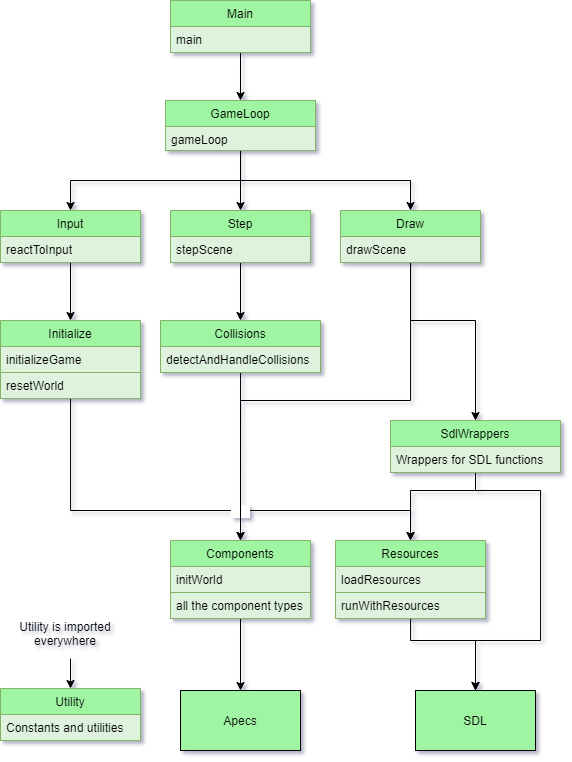
\includegraphics[width=\textwidth]{images/modules.png}
    \caption{hAsteroids module structure.}
    \label{fig:hasteroidsmodules}
\end{figure}


% components
\subsection{Components in hAsteroids}
There are more approaches to designing components, but in hAsteroids,
we have three categories of components: \say{marker} components,
\say{shared} components, and \say{control} components. Marker components serve two purposes:
they contain information that is unique for a given type of game object,
and that way, they also mark an entity as that object.
Shared components include characteristics that are shared by more types
of game objects like position. Lastly, control components are all global
and are used in one way or another to control the run of the game and the transitions between scenes.
hAsteroids has one \inlinehs{Unique} marker component called \inlinehs{Ship},
which marks an entity representing the player's ship and stores
the angle of the direction the ship is facing. The three other marker
components are \inlinehs{Map} stored. They are \inlinehs{Asteroid} — holding
asteroid size — \inlinehs{Ufo} — holding saucer size and a countdown
to the next UFO's shot being fired — and \inlinehs{Bullet} — storing whether
the player or a UFO shot it. Next, there are the shared components
\inlinehs{Position}, \inlinehs{Velocity} and \inlinehs{TimeToLive}
and several \inlinehs{Global} control ones like \inlinehs{ShipLives},
\inlinehs{ShipState}, \inlinehs{GameLoopState}, \inlinehs{WaveTime} and few others.
Table \ref{tab:entities} shows which game object types should have which components,
however, it can't be enforced by types due to the nature of ECS.

\begin{table}[hbt]
  \begin{tabularx}{\textwidth}{|r|X|}
    \toprule
    Object & Components \\
    \midrule
    % Ship     & \inlinehs{Position}, \inlinehs{Velocity}, \inlinehs{Ship} \\
    % UFO      & \inlinehs{Position}, \inlinehs{Velocity}, \inlinehs{TimeToLive}, \inlinehs{Ufo} \\
    % Bullet   & \inlinehs{Position}, \inlinehs{Velocity}, \inlinehs{TimeToLive}, \inlinehs{Bullet} \\
    % Asteroid & \inlinehs{Position}, \inlinehs{Velocity}, \inlinehs{Asteroid} \\
    Ship     & {Position}, {Velocity}, {Ship} \\
    UFO      & {Position}, {Velocity}, {TimeToLive}, {Ufo} \\
    Bullet   & {Position}, {Velocity}, {TimeToLive}, {Bullet} \\
    Asteroid & {Position}, {Velocity}, {Asteroid} \\
    \bottomrule
  \end{tabularx}
  \caption{Game objects and their components.}
  \label{tab:entities}
\end{table}


% the outer level
\subsection{Initialization and looping}
\label{sect:initialization}
The \inlinehs{main} function is the entry point of the program. It first initializes
the SDL libraries and then creates a window and a renderer. Next, using \inlinehs{loadResources},
it loads object textures into a hash map, prerenders fonts saving them into another
hash map and wraps it all together with the renderer and a few stateful random generators
into one product type called \inlinehs{Resources}. Then the game world with our
components is created by calling \inlinehs{initWorld}, and together with resources,
they are passed to the \inlinehs{gameLoop} through a stack
of monad transformers (\inlinehs{SystemWithResources}). When the gameLoop quits,
the window is destroyed, resources are freed.


% Systems
\subsection{Systems in hAsteroids}

\inlinehs{gameLoop} is one large compound system responsible for \textbf{updating} and \textbf{drawing}
the world and the menus every frame of the game. World updating is split
into two functions: \inlinehs{reactToInput} and \inlinehs{stepScene}.
The scene (a menu or the world) is then drawn by \inlinehs{drawScene}.
It also measures elapsed time every frame and calls \inlinehs{SDL.Delay} if it was
updated and drawn too quickly for the targeted 60 FPS.
This is then repeated until the player quits the game.

\subsubsection{\textbf{Reacting to input}}
\inlinehs{reactToInput} manages the state of the input, and as its name suggests,
reacts to it. Depending on the global \inlinehs{GameLoopState} component,
it either transitions between the states (\inlinehs{InMenu}, \inlinehs{Playing},
\inlinehs{Paused}, \inlinehs{GameOver}, \inlinehs{Quit}) or
when in the \inlinehs{Playing} state, it also allows the player to control the ship.
That is done by a \inlinehs{cmapM} which changes the angle of the ship,
increases its velocity or creates a new bullet entity --- all conditioned by the input state.

\subsubsection{\textbf{Stepping the scene}}
\inlinehs{stepScene} takes care of simulating physics and game rules
over time when the loop is in the \inlinehs{Playing} state.
This is divided into a series of twelve function calls:

\begin{itemize}[\textendash]
    \item  \inlinehs{cmap $ stepKinetics dT}\\
    iterates over all entities and adds their velocity vector multiplied
    by time \inlinehs{dT} to their position vector and also takes care
    of wrapping the space — if an entity flies out of the screen on one side,
    it comes back in from the other side.

    \item \inlinehs{cmap $ decelerateShip dT}\\
    simply applies deceleration to the ship by scaling down its velocity vector slightly.

    \item \inlinehs{cmapM $ stepShipState dT}\\
    is responsible for transitioning between ship states
    (\inlinehs{Alive}, \inlinehs{Exploding Int}, \inlinehs{Respawning Int},
    where the integers serve as countdown timers for the state transition)
    and the explosion animation.

    \item \inlinehs{cmapM_ $ ufosShoot dT}\\
    iterates over all \inlinehs{Ufo} components decrementing the time to
    shoot and when it reaches 0, it creates a new \inlinehs{Bullet}.
    The algorithm for finding a shooting direction is different for the two UFO sizes.
    Small UFOs are more accurate because the algorithm uses
    the law of sines to calculate the bullet trajectory based on the ship's current
    position and velocity. Large UFOs shoot in quarter of $\pi$ increments
    towards the ship's current location.

    \item \inlinehs{awardLifeIf10000}\\
    increments ship's lives by 1 for reaching every 10000 score points.

    \item \inlinehs{modify global $ \(WaveTime t) -> WaveTime $ t + dT}\\
    simply adds the frame delta time \inlinehs{dT} to the wave time counter.

    \item \inlinehs{spawnUfos}\\
    randomly creates new UFO entities on the left side of the screen,
    with the chances increasing as the time spent in one wave (\inlinehs{WaveTime}) passes.

    \item \inlinehs{spawnNewAsteroidWaveIfCleared}\\
    uses \inlinehs{cfold} from Apecs to count all asteroids and
    when there are none it starts counting up using the \inlinehs{WavePauseTimer}.
    When the timer reaches 1500 it calls \inlinehs{spawnNewAsteroidWave}
    from the \inlinehs{Initialize} module, which uses the random stateful
    generators from the \inlinehs{WithResources} reader monad to create new asteroids.

    \item \inlinehs{cmap $ \(Ttl t) -> Ttl $ t - dT}\\
    simply subtracts the frame delta time \inlinehs{dT} from all the
    \inlinehs{TimeToLive} components.

    \item \inlinehs{destroyDeadBullets} and \inlinehs{destroyDeadUfos}\\
    use \inlinehs{cmapM_} to destroy all the components for entities that run out of \say{time to live}.

    \item \inlinehs{detectAndHandleCollisions}\\
    is defined in its own module \inlinehs{Collisions}.
    There the collisions are detected and handled individually between each
    entity group. The general idea is that we use \inlinehs{cmapM_} inside of \inlinehs{cmapM_}
    as an equivalent of nested for loops. This way, for every asteroid,
    we iterate (or map) over all the other entities, checking for collision.
    We do the similar for the rest of the combination pairs,
    using in total $\binom{6}{2} = 6$ algorithms. All the collisions are detected
    simply as a question of \say{is a point or any of the points inside of a rectangle,
    an ellipse or a circle.} A detected collision always results in some effect
    --- the colliding entities are removed, except an asteroid may break into two
    smaller ones if it is not already the smallest size, and
    in the case of the ship, one life is subtracted.
\end{itemize}

\subsubsection{\textbf{Drawing the scene}}
Once the scene is stepped, it is then \textbf{drawn} by the already mentioned \inlinehs{drawScene}
function from the \inlinehs{Draw} module. If the loop state is \inlinehs{InMenu} or
\inlinehs{GameOver} only text is drawn on a cleared black screen. That is done by
\inlinehs{drawCenteredTexts}, which only calls a monadic \inlinehs{zipWith} with
\inlinehs{drawCenteredText} on a list of y coordinates and a list of text keys.
\inlinehs{drawCenteredText} itself then looks up the text texture in the
hash map that is part of the \inlinehs{WithResources} environment,
queries its width and finally calls \inlinehs{drawText} with the coordinates
for the texture to be drawn centered.

When the loop is in the \inlinehs{Paused} state, there is text being drawn
as well as the world. Naturally, when the state is \inlinehs{Playing},
only the world is drawn. This is taken care of by \inlinehs{drawWorld},
which calls functions to draw the background, entities and the UI
(number of lives and the score). Entities are drawn using \inlinehs{cmapM_}
with a lambda function and a wrapper function around the \inlinehs{SDL.copy} and
\inlinehs{SDL.copyEx}, which renders the corresponding texture for every entity.


% Reflection
\section{Reflection}
\label{sect:apecsreflection}

From this example alone,
we learn that Apecs makes game programming in Haskell surprisingly accessible.
Once we understand the ECS principle, every world modification is
\say{intuitively imperative} thanks to the \inlinehs{SystemT w m a} monad and
the component map functions. Any system side effects can be added
to an existing \inlinehs{cmap} call with a simple change of the return types
as demonstrated in listing \ref{lst:changingmind}
\begin{listing}[H]
\begin{haskell}
-- steer and thrust
handleInput input =
    cmap $ \(Ship a, Velocity vel) ->
               ( Ship $ a + steering input
               , Velocity $ vel + thrust input a
               )
-- we realized that we also want to be able to pause the game
handleInput' input =
    cmapM $ \(Ship a, Velocity vel) -> do
                when (wasPressed input escapeKeycode)
                    (set global Paused)
                pure ( Ship $ a + steering input
                     , Velocity $ vel + thrust input a
                     )
\end{haskell}
\caption{We can easily switch between non-effectful and effectful calls.}
\label{lst:changingmind}
\end{listing}

Moreover, the \inlinehs{WithResources} reader monad provides easy
access to resources without having to pass them along everywhere as a function argument.

Not less important is the fact that the game works.
The development experience was smooth, with no major hick-ups.
Because Haskell is a statically-typed high-level language, there is
no reason to worry about random invalid memory access making our game crash,
and everything is type-safe.

However, this approach is far from perfect. Handling collisions on an
individual basis would scale very poorly, so some universal interface would be better.
This could be achieved by defining a class and its instances for the marker components.
More polymorphism could also differentiate functions that require the
\inlinehs{System} monad, the \inlinehs{WithResources} monad or both.
In the current state, there are many functions, such as \inlinehs{reactToInput},
which do not use the resources but still have access to them since
everything returns the transformed \inlinehs{SystemWithResources} monad
that has \inlinehs{WithResources} inside of it. Furthermore,
said monad transformer stack\footnote{
\inlinehs{type SystemWithResources = SystemT World (ReaderT Resources IO)}
where \inlinehs{SystemT} is only a \inlinehs{newtype}
around \inlinehs{ReaderT} defined in Apecs
}
includes \inlinehs{IO}, so any function with this type can perform
input or output effects, which goes against functional purity and nullifies
many of the reasons why one would choose Haskell as a language in the first place.

Another issue we observe is partially tied to the nature of ECS — there
is no way to destroy all of entity's components automatically in Apecs.
One has to do destroy them explicitly. That way, nothing protects us
from accidentally adding a component to an entity that will never be destroyed.
This could be mitigated by creating helper functions for entity creation and destruction.

Overall, because Apecs is so powerful, it makes it easy for the programmer to rely
on it too much and produce code that does not reach all the potential
benefits of purely functional programming.



% ====================================
% CHAPTER 3 - About functional style
% ====================================

\chapter{Focusing on functional purity --- pure-asteroids}
\label{chptr:purity}

\section{Game engines in purely functional style}
\label{sect:pureengines}

In the previous chapter we see how a program in Haskell can still be
written in a very imperative style. 
This is certainly a valid approach and has its benefits as we discuss
further in chapter \ref{chptr:evaluation} but for the second version of
Asteroids (project \emph{pure-asteroids}) we focus on functional purity,
clarity and proper compartmentalization.

The design is inspired by a keynote\cite{carmackkeynote} of John Carmack, the co-founder
of id~Software and co-creator of the Doom and Quake games.%\cite{carmackbio}
At one point in the keynote he talks about how he had been moving towards
a functional style of programming with \cpp{} and seeing the long term benefits.
He also talked about his experiments with Haskell and his vision for multi-core
game logic. \say{State of where we're at right now with game code, is that we run
all the game code in one thread because the idea of using locks to synchronize
amongst all of our current game code was just absolutely terrifying,} he says and
continues to explain how independent parallelism is much more feasible with pure
functions and how events can be used for interactions between the isolated groups.

The world-updating function can be split into individual sub-functions that update each group
of entities. Each sub-function is passed the game world and the group of entities and
it returns the updated group, therefore, in Haskell, such function cannot affect
anything outside of the group it returns. For that reason, it could be easily run
in parallel, increasing the performance.

With this approach, comes one more advantage
--- all entities are being updated based on the same image of past state, meaning
it does not matter in what order entities are updated, the result will be the same.
This can be contrasted with a naive imperative approach, where entities are
updated sequentially in-place based on the current state. Such approach may lead to
inconsistencies if for example two units attack each other at the exact same time.
Or to give an example from Asteroids, if a UFO and the ship shoot at each other
with an asteroid in between them, whichever bullet's collision is detected first
would destroy the bullet and the asteroid and the other bullet would fly through
killing either the UFO or the ship. However, the opposite approach comes with a caveat
and that is the issue of two objects moving into a common space when they are not allowed to overlap.
John Carmack addresses this in his already mentioned keynote\cite{carmackkeynote} and
says it can be solved for instance by some kind of repulsion force. Fortunately, this
is a non-issue in Asteroids because all objects may overlap, usually causing a collision
and destruction.



% Writing of
\section{Writing of pure-asteroids}
\label{sect:pureimplementation}

\begin{figure}[hbt!]
    \centering
    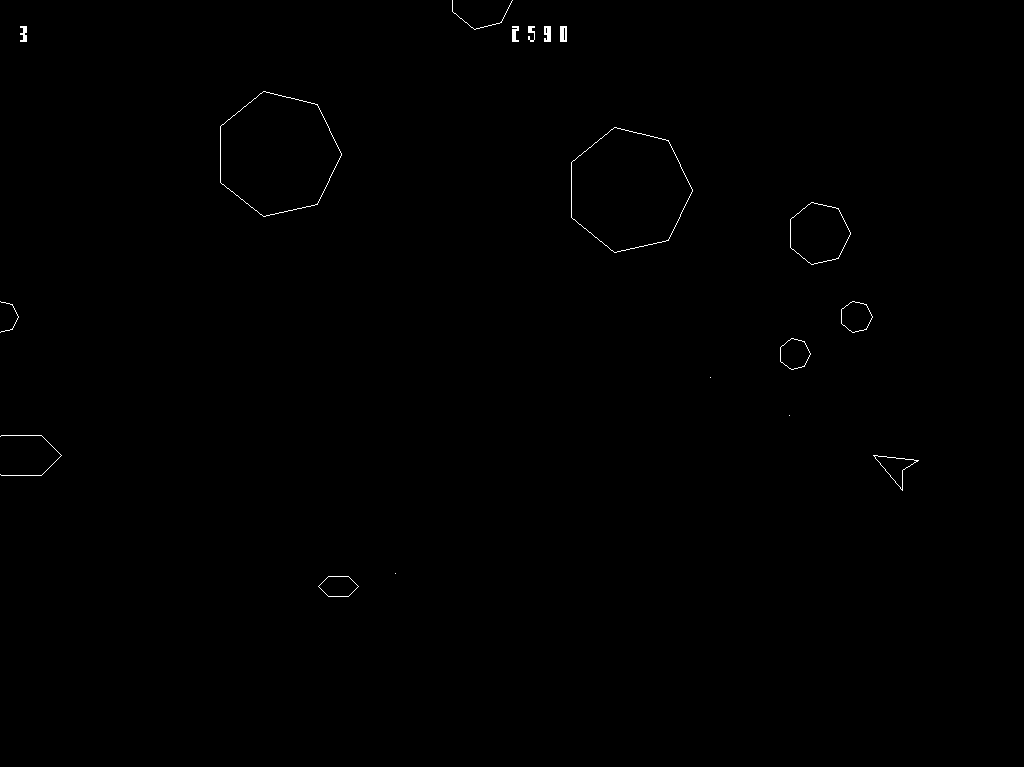
\includegraphics[height=5cm]{images/pure-screenshot.png}
    \caption{A screenshot of pure-asteroids game-play.}
    \label{fig:pureasteroidsscreenshot}
\end{figure}

In this section we describe how \emph{pure-asteroids} implements a pure style engine described
in the \hyperref[sect:pureengines]{previous section}.
The program's main function is very similar to the one from
hAsteroids with the exception of texture loading because pure-asteroids
draws vector graphics using \inlinehs{drawScene}. There is also no reader monad
and \inlinehs{gameLoop} is passed everything explicitly as arguments.
The looping itself is also very similar to hAsteroids but naturally,
the world updating and drawing differs. The world state passes through
\inlinehs{processWorldEvents}, which fulfils all the requests from events,
through \inlinehs{stepWorld}, which simulates physics and game rules and generates new events,
\inlinehs{drawScene} draws it and \inlinehs{resetIfNewGame} returns a reinitialized
world only if the loop state is transitioning from \inlinehs{InMenu} to \inlinehs{Playing}.
This is illustrated in figure \ref{fig:worldeventsflow}.
\begin{figure}
    \centering
    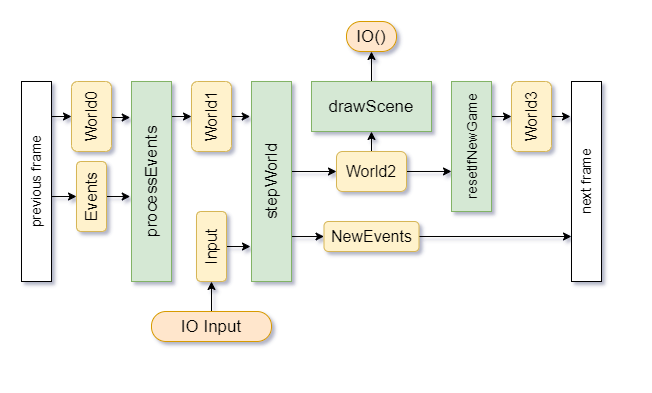
\includegraphics[width=\textwidth]{images/world-flow-detailed.png}
    \caption{Data flow of \inlinehs{gameLoop}.}
    \label{fig:worldeventsflow}
\end{figure}
Next, we describe the used \textbf{data structures} and then explain
how the \textbf{stepper function} and \textbf{event processing} use them.
% \begin{figure}
%     \centering
%     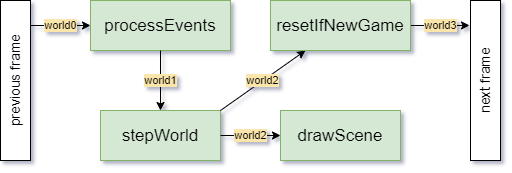
\includegraphics[width=\textwidth]{images/world-flow-basic.png}
%     \caption{The flow of world sate variable.}
%     \label{fig:worldflow}
% \end{figure}


\subsection{Data structures}
The two main data structures, as already shown in figure \ref{fig:worldeventsflow},
are the world sate represented by \inlinehs{World} and the events for communication
between entity groups represented by \inlinehs{WorldEvents}.

The definition of \inlinehs{World} can be seen in listing \ref{lst:pureworld}.
\inlinehs{World} contains separate groups of entities and some other state variables.
\inlinehs{Asteroids}, \inlinehs{Ufos} and \inlinehs{Bullets} are type
aliases for hash maps of the respective entities.
The entities themselves then contain similar data as components in hAsteroids,
only here, the data is all in one place, grouped by the game object.
Listing \ref{lst:pureship} shows \inlinehs{Ship} definition as an example.
We can notice the preceding underscores in the record names. This is used
to generate lenses by using \inlinehs{makeLenses} from the \packagename{mtl} package
to facilitate easier data manipulation in our nested structures.

% Game World
\begin{listing}[H]
\begin{haskell}
-- | Game world state structure 
data World =
    World
    { _wShip      :: Ship 
    , _wAsteroids :: Asteroids
    , _wBullets   :: Bullets
    , _wUfos      :: Ufos
    , _wWaveTime  :: Time
    , _wWavePause :: Time
    , _wWaveNum   :: Int
    , _wScore     :: Score
    }
\end{haskell}
\caption{World structure in pure-asteroids.}
\label{lst:pureworld}
\end{listing}

% The Ship and its state
\begin{listing}[H]
\begin{haskell}
-- | Ship state structure
data Ship =
    Ship 
    { _sPosition :: Position
    , _sVelocity :: Velocity
    , _sAngle    :: Angle
    , _sLives    :: Int
    , _sState    :: ShipState
    }

data ShipState
    = ShipAlive
    | ShipExploding Time
    | ShipRespawning Time
\end{haskell}
\caption{The \inlinehs{Ship} representation in pure-asteroids.}
\label{lst:pureship}
\end{listing}

Listing \ref{lst:events} shows the event package type \inlinehs{WorldEvents}.
It also has an instance of \inlinehs{Monoid}, which allows us to collect the packages from
each entity group and combine them into one in the \textbf{stepper function}
and then we distribute the events to their addressed entity groups in \textbf{event processing}.
The individual event types and the information they carry are described later,
with the functions that process them.

% World Events type
\begin{listing}[H]
\begin{haskell}
-- | Structure for event passing between entity groups
data WorldEvents =
    WorldEvents
    { _forAsteroids :: [AsteroidEvent]
    , _forShip      :: [ShipEvent]
    , _forUfos      :: [UfoEvent]
    , _forBullets   :: [BulletEvent]
    , _forScore     :: [ScoreEvent]
    }
\end{haskell}
\caption{The event package structure.}
\label{lst:events}
\end{listing}


% stepWorld
\subsection{Stepper function}
We can see the combining of event packages happen in the definition of \inlinehs{stepWorld}
in listing \ref{lst:purestepworld}. The events are returned by
the individual steppers of each entity group together with the stepped versions
of those groups. Note how lenses are used to \say{focus} on the contents of world state
and change them with the setter operator \inlinehs{.~} or the function applicator \inlinehs{%~}
(or also the lens equivalent of \inlinehs{+=}).
Each \say{substepper} is compartmentalized and could be made to run in parallel.

% stepWorld definition
\begin{listing}[H]
\begin{haskell}
-- | Update the world
--   simulating physics and reacting to input
stepWorld :: Time -> InputState -> RandomStream Double -> World -> (WorldEvents, World)
stepWorld dT input rand oldW =
    let
        (eventsS, newShip)    = stepShip dT input oldW $ oldW ^. wShip
        (eventsB, newBullets) = stepBullets dT input oldW $ oldW ^. wBullets
        (eventsU, newUfos)    = stepUfos dT rand oldW $ oldW ^. wUfos
        (eventsScr, newScore) = stepScore dT $ oldW ^. wScore
    in
        (,) (eventsS <> eventsB <> eventsU <> eventsScr) $
        checkWave $
        oldW
          & wShip      .~ newShip
          & wAsteroids %~ stepAsteroids dT
          & wBullets   .~ newBullets
          & wUfos      .~ newUfos
          & wWaveTime  +~ dT
          & wScore     .~ newScore
\end{haskell}
\caption{The stepper function.}
\label{lst:purestepworld}
\end{listing}

Figure \ref{fig:entitygroups} shows which events, represented by their data constructors,
entities may send to others.
The working of the individual \say{substeppers} can be summarized as follows:
\begin{itemize}
% TODO
    \item \inlinehs{stepShip}\\
    does things \# TODO.

    \item \inlinehs{stepAsteroids}\\
    does things \# TODO.

    \item \inlinehs{stepBullets}\\
    does things \# TODO.

    \item \inlinehs{stepUfos}\\
    does things \# TODO.

    \item \inlinehs{stepScore}\\
    does things \# TODO.
\end{itemize}
After that, \inlinehs{checkWave} takes care of spawning new waves of asteroids
and then the stepped world is paired with the generated events and returned.

% Entity interactions figure
\begin{figure}
    \centering
    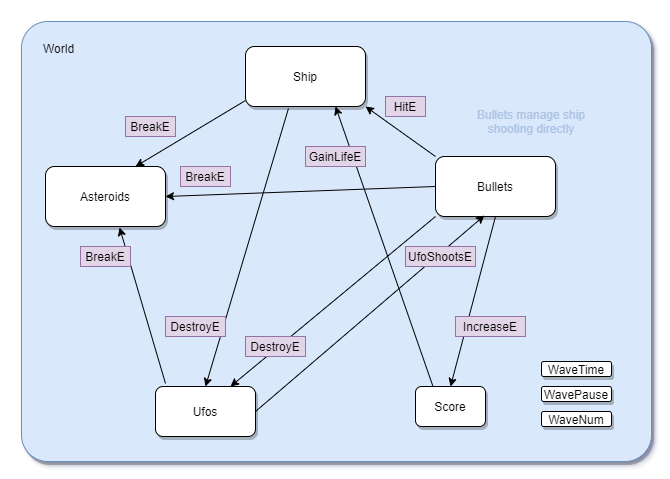
\includegraphics[width=\textwidth]{images/entity-relationships-transparent-bg.png}
    \caption{Entity groups and their interactions.}
    \label{fig:entitygroups}
\end{figure}


\subsection{Event processing function}

% processWorldEvents definition
\begin{listing}
\begin{haskell}
-- | Process all WorldEvents
processWorldEvents :: WorldEvents -> World -> World
processWorldEvents events world =
    world
      & wAsteroids %~ processAsteroidsEvents
                        (events ^. forAsteroids)
      & wShip      %~ processShipEvents
                        (events ^. forShip)
      & wUfos      %~ processUfosEvents
                        (events ^. forUfos)
      & wBullets   %~ processBulletEvents
                        (events ^. forBullets)
      & wScore     %~ processScoreEvents
                        (events ^. forScore)
\end{haskell}
\caption{The event processing function.}
\label{lst:pureprocessevents}
\end{listing}

% TODO also fix indentation
In listing \ref{lst:pureprocessevents} we can see the implementation of
event processing and again the use of lenses.
Similarly to \inlinehs{stepWorld}, the work is compartmentalized
and could be made to run in parallel.
% TODO
\# TODO maybe \{itemize\} the description of subfunctions,
maybe don't, and describe the individual event types too


% Reflection
\section{Reflection}
\label{sect:purereflection}

Overall, pure-asteroids achieves what it sets out to do --- we can observe
many of the benefits described in section \ref{sect:whyfpmatters}.
Because it uses less abstraction, the code is safer and more expressive.
For example, by looking at \inlinehs{shoot} from the \inlinehs{Step.Bullets} module
\begin{haskell}
shoot :: InputState -> World -> Bullets -> Bullets
shoot input w =
    if wasPressed input spaceKeycode
        then insertBullet
        else id
\end{haskell}
We immediately see from the name and the type signature that the function presumably
somehow alters the collection of \inlinehs{Bullet}s based on the input and that
the alteration is probably adding a new bullet, which is confirmed by looking
at the next four lines of light code. And this also means that it is \emph{the only thing}
the function can do --- it clearly can't change the state of the ship, read from a file
or render a white square.

It also incorporates what we may call \say{functional elegance}.
Throughout the code base, we use functions like \inlinehs{map}, \inlinehs{filter},
\inlinehs{fold}, \inlinehs{traverse} and many others, that Haskell programmers are familiar
with and which make the code brief and save us time.

Most importantly, as we demonstrated, the design could be adapted to
use parallelism, which we expect would increase performance.
Parallel computation would be especially beneficial if the game was of larger scale
and the computation was more demanding --- for instance collision detection
in pure-asteroids is very simple but it could be improved by using more
complicated algorithms.

However, even though we could use parallelism, the scalability of our design is somewhat lacking.
It would be appropriate to use more classes in general. A class interface for
collision detection, stepping, communication using events and for resources abstraction.
Pure-asteroids is too explicit, which makes it relatively rigid
--- adding a random number
generator to a bottom-level function, requires passing it from the top level
as an argument through the whole function chain. And the long type signatures of the
top-level functions make them actually less clear.

Ultimately, we see that explicitness is good but has its boundaries,
and that some level of abstraction is needed. 
It should be also pointed out that designing the complete engine from scratch
was a significant amount of effort, despite the development being smooth and the final
product working well.




% ========================================
% CHAPTER 4 - Analysis of imperativness
% ========================================

\chapter{Analyzing an existing \cpp{} implementation}

\section{}
Explain a bit about the choice of the particular implementation and
comment on the quality of code

the options turned out to be not so great, like my implementations
this version is not flaw-less. we point out its mistakes and present
them as a possible outcome of this language choice, although the choice
definitely does not need to imply them nor conditions them
-> there can be a great program in \cpp{} and a really bad one in Haskell.

\section{}
outline its working and architecture

\section{}
reflect on it

in a way very intuitive - objects, \say{imperatives}

good scalability in terms of adding new entities or features,
however there should be separate manager classes for entities

some whoopsies - valgrind shows memory leaks and uses of uninitialized values

effects can be everywhere -> high flexibility low safeness

...maybe this chapter could be a section in \textbf{Comparing the approaches}




% ====================================
% CHAPTER 5 - Final COMPARISON
% ====================================

\chapter{Evaluation of the approaches}
\label{chptr:evaluation}

in this chapter we first compare the three implementations, paying attention to modularity,
expressiveness, safeness, development costs and performance.
Then we discuss the conflicts observed in the comparisons
and reflect on weather the promised benefits of Haskell from section \ref{sect:whyfpmatters}
were reached.

note: replace "safeness" with "security"?

\section{Comparison}
% TODO: show a part of code where hAsteroids looks close to the c++

address how this is not meant to be an evaluation of imperative languages,
even though we are comparing against them and critiquing them
--- especially against \cpp{} which does not fully represent all the imperative languages

\subsection{Flexibility and scalability}

Both \textbf{hAsteroids} and \textbf{imperative asteroids} are very flexible designs.
Because in hAsteroids, the monad return type of most functions is not very
restrictive at all, we can add in and take away effects or resources with ease.
Similarly the imperative version is highly flexible in this sense. When it comes
to scalability, both do decently well. Adding new game objects in hAsteroids can be done by
defining more components and needed systems. Already existing components and systems can be reused
like \inlinehs{Position}, \inlinehs{Velocity} and \inlinehs{stepKinetics}.
One issue would be the expansion of collision detection,
which is done on an individual basis, therefore the amount of work
would grow linearly with increasing number of game objects.
Imperative Asteroids do better in this regard --- kinetic properties can
be inherited from \inlinecpp{FlyingObject} as well as the ability to detect collisions.
The issue there might be if we wanted to inherit only parts of \inlinecpp{FlyingObject}.
Also with large scale, the safeness becomes more of a concern for both games
--- more on that in the following subsection.

We have already described how \textbf{pure-asteroids} are rather rigid because of
their lack of abstraction. Scalability is also worse than the other two, since
adding new objects would require writing their whole \say{substepper} and
new event paths, and collision detection is handled similarly to hAsteroids.

\subsection{Expressiveness and safeness}

As we have already discussed in chapter \ref{chap:motivationandmethods},
functional languages are designed to be clearer (\emph{expressiveness})
and to have better control of side effects (\emph{safeness}) then conventional
imperative languages. Now the imperative code can be even more or less unsafe
depending on its type system. \cpp{} is mostly strongly and statically typed, which
does provide a certain amount of assurance, some other languages are not.
This can protect us from trying to add an object to a number for instance.

Many languages also take various steps towards controlling side effects.
One such example could be the \inlinecpp{const} keyword used to define a variable
that cannot be mutated. In \cpp{} this keyword can also be used on methods
to prevent them from changing the state of the object, allowing us to call these
methods even on \inlinecpp{const} objects. Usage of this keyword, would prevent
the author of imperative asteroids from writing this drawing function that
unexpectedly also changes the state of bullets:
\begin{cppblock}
void Game::draw(const Interface &ui) {

    /* ... other objects are drawn... */
    
    for (int i = 0; i < bullets.size(); i++) {
        if (bullets[i]->isAlive()) {
            bullets[i]->draw();
            bullets[i]->setHealth(); // a setter?!
        }
    }
}
\end{cppblock}
However, languages like Java or Python do not support immutable objects
and we can see how control of side effects in general is a \say{plan B} in the imperative paradigm.

Conversely, since Haskell originated as an academic language,
functional purity was allowed to be plan A and having
side effects was actually the plan B in this case. We saw how this works out well for expressiveness
in the example of \textbf{pure-asteroids} as showcased at the beginning of section \ref{sect:purereflection}.
And because all variables are immutable, change is made explicit as a \emph{new} returned value
that we pass forward.
Moreover, any input/output side effects are clearly separated by the \inlinehs{IO} monad
and the rest of the code is completely deterministic, which all together with strong static typing
makes for a very safe language.

That is, if used well --- \textbf{hAsteroids} turned out to be a very interesting game.
Apecs makes game programming in Haskell approachable and provides
very good performance by being \emph{strict and imperative}. This inner imperativness
makes purity sort of a plan B again, and the programmer has to be clever about using monad polymorphism
if they want to keep \say{the danger of \inlinehs{IO}} contained. This has occurred to us in the middle
of the hAsteroids development process and so we decided to embrace it and see where it leads.
If we redesigned the types we could have reached better safeness and even expressiveness, however,
with the game world sate abstracted it is still not always clear what functions do
when applied through \inlinehs{cmapM} or \inlinehs{cmapM_}.



\subsection{Development costs}

- development speed and comfort

- ease of testing and debugging\\
how do you test this:
\begin{cppblock}
// Move each of the bullets forward if it is alive
void Game::advanceBullets() {
    for (int i = 0; i < bullets.size(); i++) {
        if (bullets[i]->isAlive()) {
            bullets[i]->advance();
            if (!isOnScreen(bullets[i]->getPoint())) {
                bullets[i]->kill();
            }
        }
    }
}
\end{cppblock}
how OOP objects model state of their methods

\subsection{Performance}

do benchmarks profiling if time


% \subsection{pure-asteroids \vs imperative Asteroids}

% \subsection{pure-asteroids \vs hAsteroids}

% Both implementations are technically functional and both technically separate
% pure code from impure code with \inlinehs{IO}. But we have already mentioned
% how hAsteroids does not leverage the type system to do so.

% \subsection{hAsteroids \vs imperative Asteroids}

% They are surprisingly similar.

% The difference (or lack there of??) between monad state and an implicit object state.
% Separation of effectful and uneffectful code - monad and const keyword.

% Haskell can be a very imperative language

\subsection{Code statistics}
Some statistics about code length and keyword usage perhaps here for fun


% Further discussion about programming theory
\section{Observed dilemmas}

\subsection{Flexibility \vs safeness}

\subsection{Abstraction \vs expressiveness}

\subsection{...?}


% RECAP and final EVALUATION
\section{Recapitulation / Final lesson}

it is said that Garbage Collection (GC) can be a problem in Haskell
with interactive real-time applications like video games, but it has been proven that
it is ok for small to medium sized games
--- paradox: pure functional design is great for long term and large scale,
with Haskell the upfront cost is higher but the system produced is more likely to be of high quality

classes can (and should) be used for polymorphism, increasing flexibility scalability and
reducing code duplicity

it remains to be true even for game development that the code can be more expressive,
safer and briefer --- there is a balance between abstraction and explicitness

the language it self being very high-level and abstract can make it much more
difficult to optimize, which is important for games --- languages like \cpp{} have the advantage

We have rediscovered that Haskell can be very imperative, as explained by Simon P.~Jones and
Philip Wadler in their paper \textit{Imperative Functional Programming}.\cite{imperativefp}
% https://www.microsoft.com/en-us/research/wp-content/uploads/1993/01/imperative.pdf
% https://youtu.be/re96UgMk6GQ?t=2089
In that paper, they described for the first time, how monads could be used for input/output operations
in lazy languages, and confirmed what we see in hAsteroids ---  with the \inlinehs{IO} monad
Haskell can very closely resemble C. Yet, it keeps the benefits of functional style intact by
clearly separating the imperative from the functional.

perhaps also quote Carmack again, when he said how over the years of supervising
hundreds of programmers working of thousands and thousands of lines of code, he saw that
anything that is legal for the compiler will end up in your code base eventually
--- Haskell's "brutal" functional purity is a win



% TEMP notes
\chapter*{Temporary notes on comparing}

These are other ways of structuring the comparison. Please, excuse the mess.

\section{Common game engine features}
here we compare the already described games by how they
deal with the common needs of a game

\subsection{Data modelling}
how data is modeled --- we have an example of ECS, "struct" collections
and object collections (in OOP data is modelled as objects together with related functionality)

ECS - data locality and component design - fast and flexible

struct collections - compartmentalization - safe and could be made to run in parallel

object collections - 

\subsection{Input handling}

in pure-asteroids we keep a input state variable and then pass it to the stepper function

in hAsteroids and the imperative version it is an effectful code
--- \emph{difference between a state monad abstraction and the state of an object}

\subsection{World stepping}

again pure-asteroids sends an explicit world state variable through functions

hAsteroids with ECS a sequence of 12 calls - could be grouped but the
changes are still across components not objects

the imperative version iterates over the collections and calls \inlinehs{advance()},
for some reason \inlinehs{draw()} increments the asteroid rotation
--- \emph{the line between freedom and safeness}

consistency - with apecs the result could differ based on the order in which
entities are iterated over (\# todo - make sure it is that way + apecs-stm solves this (?)),
pure-asteroids naturally step regardless of order and imperative asteroids use a flag to mark
objects for destruction and then do it later

\subsection{Detecting and handling collisions}



\subsection{Output handling}

in pure-asteroids the drawScene is the only impure part of \inlinehs{gameLoop},
besides event polling, time measuring and calling a delay. it cannot alter the world

in apecs \inlinehs{cmapM_} gives us an almost safe almost read only access to world,
but other \inlinehs{cmap} can be used inside of it so not very safe

imperative version, unfortunate design choice, \inlinehs{Game.draw()} not only draws
but also increments asteroid rotation and decrements bullet health (that is used as time to live)
and it even flags bullets as dead if health reaches 0

\section{Attributes}
We evaluate our described implementations based on several desirable attributes for video games,
some of which were promised in section \ref{sect:whyfpmatters} as benefits of Haskell.

aspects of Modularity:
\subsection{Flexibility and scalability}


\subsection{Briefness and development speed}

Haskell has interpreter but can also be compiled -> fast development \emph{and} fast programs

Haskell code is often said to be much shorter than its imperative equivalent.\\
\~here are some statistics, take it for what it is worth...\~\\
number of lines, words, characters\\
\mintinline{console}{wc --help}: "A word is a non-zero-length sequence of characters delimited by white space"\\

hAsteroids
\begin{term}
~/ba-thesis/hAsteroids$ wc -lwm src/*.hs app/Main.hs
  207   844  6609 src/Collisions.hs
  185   717  5380 src/Components.hs
  135   437  3551 src/Draw.hs
   46   165  1229 src/GameLoop.hs
   64   227  1854 src/Initialize.hs
  132   647  4811 src/Input.hs
  245   803  7054 src/Resources.hs
   57   219  1603 src/SdlWrappers.hs
  175   874  5969 src/Step.hs
   99   356  2583 src/Utility.hs
   67   172  1540 app/Main.hs
 1412  5461 42183 total
\end{term}

pure-asteroids
\begin{term}
~/ba-thesis/pure-asteroids$ wc -lwm src/*.hs src/Step/*.hs app/Main.hs
  149   635  4327 src/Draw.hs
   95   350  3017 src/EventProcessing.hs
  109   404  3631 src/GameLoop.hs
   58   203  1509 src/Initialize.hs
   85   384  2859 src/Input.hs
  114   381  3334 src/Resources.hs
   56   221  1862 src/Step.hs
  197   578  3975 src/Types.hs
   89   306  2013 src/Utility.hs
   17    41   315 src/Step/Asteroids.hs
  124   571  4467 src/Step/Bullets.hs
   18    87   515 src/Step/Common.hs
   24    63   468 src/Step/Score.hs
  136   667  4754 src/Step/Ship.hs
  109   540  3630 src/Step/Ufos.hs
   50   123  1167 app/Main.hs
 1430  5554 41843 total
\end{term}

Asteroids by Jason Halverson
\begin{term}
~/Asteroids$ wc -lwm *.cpp
  195   376  5416 asteroids.cpp
   78   182  2133 bullet.cpp
   45   163  1303 driver.cpp
  141   278  3043 flyingObject.cpp
  531  1549 14674 game.cpp
   67   197  1662 point.cpp
   98   228  2218 ship.cpp
  712  2805 22545 uiDraw.cpp
  331  1355 11533 uiInteract.cpp
   38    80   602 velocity.cpp
 2236  7213 65129 total

~/Asteroids$ wc -lwm *.h
  105   196  2327 asteroids.h
   36    81   790 bullet.h
   60   127  1384 flyingObject.h
  103   261  2938 game.h
   48   159  1302 point.h
   63   126  1227 ship.h
  135   580  5979 uiDraw.h
  133   644  5045 uiInteract.h
   29    62   626 velocity.h
  712  2236 21618 total

~/Asteroids$ wc -lwm *.h *.cpp | grep total
 2948  9449 86747 total
\end{term}

\# TODO: process into charts perhaps and comment on it


\subsection{Safeness and testability}
\cpp{} code needs testing more and it is more difficult to do - example...
\mintinline{cpp}{const} keyword is a very good mechanism that is not used to its
full potential in the imperative example.

Haskell has more than \mintinline{cpp}{const}, we have already pointed out how
the type of a function in pure-asteroids clearly limits its effects.
However, hAsteroids hints that poor design choices can negate this effect.

\subsection{Program performance}
with low-level languages it is easier to optimize, they don't hide
what the computer is actually doing. Haskell is \emph{very} abstract,
its formality allows the compiler to do a lot of optimizations, but
it requires deeper knowledge of \inlinehs{ghc} for the programmer
to know how the code will perform. Laziness is an example
of a language feature that can cause problems with performance...




\chapter*{Conclusion}
\addcontentsline{toc}{chapter}{Conclusion}




\printbibliography[heading=bibintoc] %% Print the bibliography.


\makeatletter\thesis@blocks@clear\makeatother
\phantomsection %% Print the index and insert it into the
\addcontentsline{toc}{chapter}{\indexname}
\printindex


\appendix %% Start the appendices.
\chapter{An appendix}
Here you can insert the appendices of your thesis.

\end{document}
